\subsubsection{Architecture}

The architecture for code generation was split into multiple components to create a compilation pipeline as outlined in \autoref{figure:code-gen-arch}.

\begin{figure}[h]
    \centering
    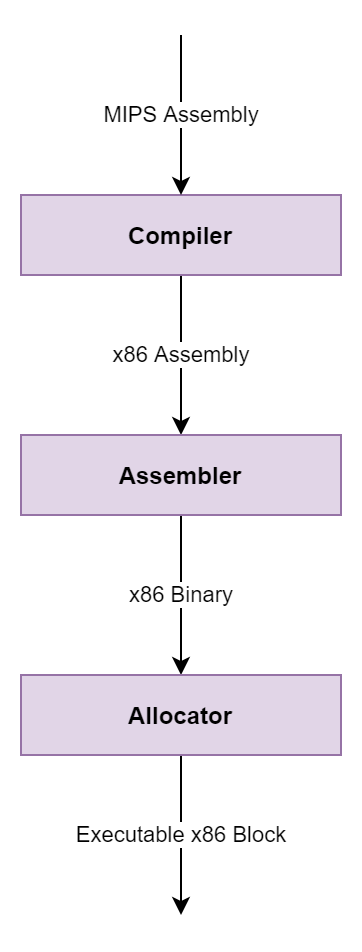
\includegraphics[width=0.25\linewidth]{diagrams/code-gen.png}
    \caption{Compilation pipeline and architecture for JIT compiling MIPS to x86.}
    \label{figure:code-gen-arch}
\end{figure}

The \texttt{Compiler} first translates the MIPS assembly to the appropriate x86 assembly. This is then converted to x86 binary by the \texttt{Assembler}. Finally, the \texttt{Allocator} allocates the appropriate executable memory for the compiled binary, producing an executable block of x86 code.

For increased performance, the \texttt{Compiler} does not actually produce an intermediate stream of x86 assembly; instead it utilises the \texttt{Assembler} to directly produce the correct x86 binary through template functions, largely minimising the runtime overhead.